% Completing the square in al-Khwarizmi (x^2 + 10x = 39)
% OrbBits TikZ conventions: see docs/style/tikz.md
\documentclass[tikz,border=6pt]{standalone}
\usepackage{amsmath,amssymb}
\usetikzlibrary{calc,arrows.meta,decorations.pathreplacing}

\definecolor{orbPrimary}{HTML}{1F5FBF}
\definecolor{orbAccent}{HTML}{E0A100}
\definecolor{orbMuted}{HTML}{7A7A7A}

\begin{document}
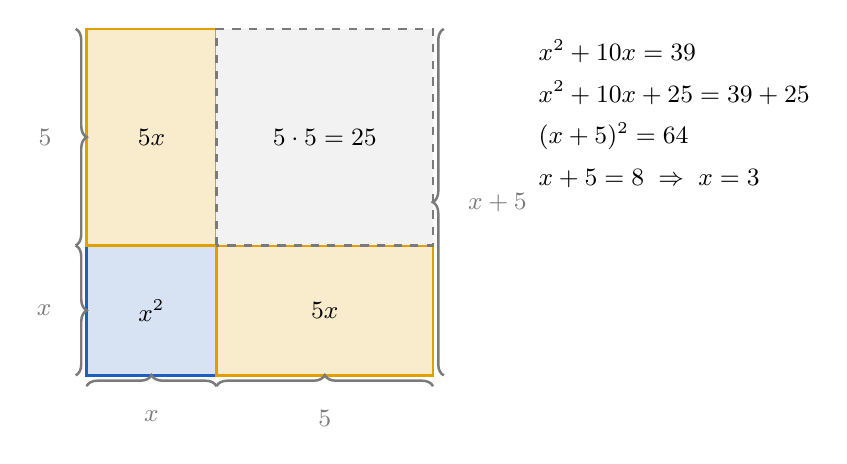
\begin{tikzpicture}[
    scale=0.55,
    line width=0.9pt,
    every node/.style={font=\small},
    brace/.style={decorate,decoration={brace,amplitude=4pt},orbMuted},
  ]
  % Geometry: x = 3 (the solution), half the coefficient = 5, total side x + 5 = 8.
  \def\x{3}
  \def\h{5}
  \pgfmathsetmacro{\s}{\x+\h}

  % The square x^2
  \fill[orbPrimary!18] (0,0) rectangle (\x,\x);
  \draw[orbPrimary] (0,0) rectangle (\x,\x);
  \node at (\x/2,\x/2) {$x^2$};

  % The two rectangles 5x (the "10x" split in two halves)
  \fill[orbAccent!20] (\x,0) rectangle (\s,\x);
  \draw[orbAccent] (\x,0) rectangle (\s,\x);
  \node at ({\x+\h/2},\x/2) {$5x$};

  \fill[orbAccent!20] (0,\x) rectangle (\x,\s);
  \draw[orbAccent] (0,\x) rectangle (\x,\s);
  \node at (\x/2,{\x+\h/2}) {$5x$};

  % The missing corner that "completes" the square
  \draw[orbMuted,dashed,fill=orbMuted!10] (\x,\x) rectangle (\s,\s);
  \node at ({\x+\h/2},{\x+\h/2}) {$5\cdot 5 = 25$};

  % Dimensions
  \draw[brace] (0,-0.25) -- node[below=5pt] {$x$} (\x,-0.25);
  \draw[brace] (\x,-0.25) -- node[below=5pt] {$5$} (\s,-0.25);
  \draw[brace] (-0.25,\x) -- node[left=5pt] {$x$} (-0.25,0);
  \draw[brace] (-0.25,\s) -- node[left=5pt] {$5$} (-0.25,\x);
  \draw[brace] (\s+0.25,0) -- node[right=5pt] {$x+5$} (\s+0.25,\s);

  % The algebra, next to the figure
  \node[anchor=north west,align=left,font=\small] at (\s+2.2,\s) {%
    $x^2 + 10x = 39$\\[4pt]
    $x^2 + 10x + 25 = 39 + 25$\\[4pt]
    $(x+5)^2 = 64$\\[4pt]
    $x + 5 = 8 \;\Rightarrow\; x = 3$};
\end{tikzpicture}
\end{document}
